\documentclass[../embeddings.tex]{subfiles}
 
\begin{document}
\subsection{Hypothesis 1: The words in closest proximity to ideologically significant words will highlight points of contention or agreement between groups and can be used for descriptive analysis.}

To test my first hypothesis I examine a list of the ten most similar words as measured by cosine similarity for each word, and a similar list for that word's counterpart from the other party. I expect that words unique to each list represent ideological divides between the parties, and common words represent points of agreement. As cosine similarity between a word and its counterpart increases, I expect that overlap between the two lists will increase. 

\begin{figure}[h]
  \centering
  \subfigure[impeach]{
  \label{fig:impeach}
  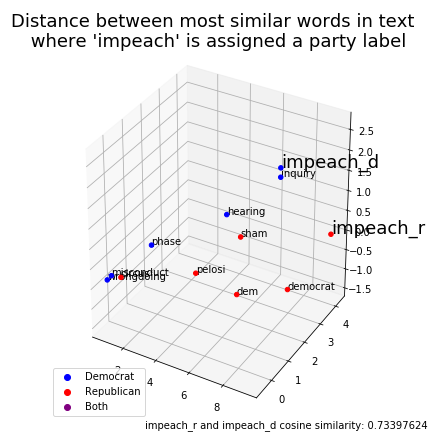
\includegraphics[width=.45\textwidth]{impeach_party}}
  \qquad
  \subfigure[robocall]{
  \label{fig:robocall}
  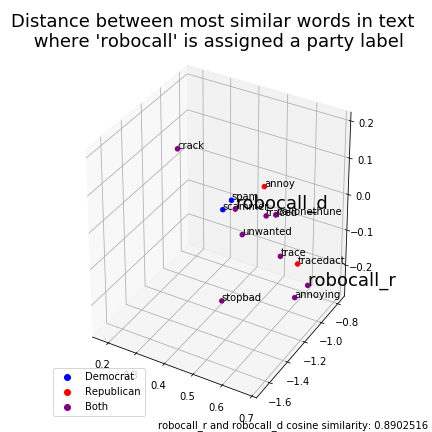
\includegraphics[width=.45\textwidth]{robocall_party}}
  \caption{PCA plots for agree and disagree words}
\end{figure}

From the disagree set of words I used the word ``impeach'' because of its relevancy to the news in the time period I collected the data. Because word vectors within the embedding contain 100 dimensions it is impossible to plot them precisely. To compensate, I applied principal component analysis (PCA) to reduce the number of dimensions \cite{scikit-learn}. PCA preforms a linear transformation on the word vectors that combines dimensions into \textit{n} principal components that explain the maximum amount of variance \cite{wold1987principal}. The result is that a word vector of 100 dimensions is reduced down to three principal components that explain the greatest possible variance. Because each component is an amalgamation of the other dimensions however, components are not readily interpretable. Rather, in this instance I use the technique solely to enable a rough visualization of the data's separation. With three dimensional PCA I am able to explain roughly 75\% of the variance between word vectors, meaning that while the plot is not an exact visualization of the distance between words, it is a decent approximation.



Figure \ref{fig:impeach} shows the scatter plot for the word ``impeach'' and the ten most similar words by party after applying PCA. The plot shows two distinct clouds for the parties with little overlap. The parties have no common terms among the ten words most similar to their version of impeach. More significantly for this hypothesis, the most similar terms clearly reflect party positions. Democratic words feature terms such as ``abuseofpower'' and ``exposethetruth'' while Republican words include ``partisan'', ``charade'', and ``circus.''

I repeated this process for the word ``robocall'' due to bipartisan legislation worked on during the data collection period to crack down on robocalls. Figure \ref{fig:robocall} showd the opposite results of ``impeach'' with significant overlap between the two versions of robocall. Most telling is that one of the closest words to the Democrat's version of robocall is the republican's version, suggesting the words are synonymous to some degree. 

Finally, the neutral word ``look'' in \ref{fig:look} exhibits what appears to be largely noise. The two words are largely synonymous as they share each other as neighbors, but other neighboring words do not appear to carry significant ideological meaning.

\begin{figure}[h]
  \centering
  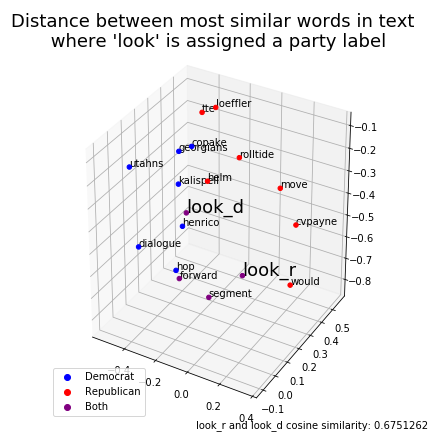
\includegraphics[width=.45\textwidth]{look_party}
  \caption{PCA plot for ideologically neutral word}
  \label{fig:look}
\end{figure}

These findings generally support my first hypothesis that word embeddings can effectively be used to provide descriptive analysis of ideological space. Notably, however, is that it is not quite as simple as my original assertion as identifying shared words. For example, in the ``robocall'' test ``annoy'' is unique to the Republican's list of words and ``spam'' is unique to the Democrats. These words do not highlight points of contention though as they generally fit with the themes of either party's list. Thus, simple heuristics may not always be appropriate and researches should exercise best judgment and domain knowledge.

\subsection{Hypothesis 2: If text is divided into two groups and separate word vectors for the same word are calculated between the two groups, that word vector will have a lower cosine similarity with its counterpart if the text is labeled by ideological group rather than labeled randomly.}

The second hypothesis is designed to test if word embeddings capture semantic differences between groups and if cosine similarity can be used to quantify those differences. Generally speaking, my expectation is that all words will have a lower cosine similarity with its counterpart when labeled by party rather than randomly, albeit I do expect the difference between party and randomly labeled data to be greatest between words that represent disagreement and smallest between words that represent agreement. I expect near universal difference because even if a word represents a point of agreement between the parties, I still expect slight variation in the party's talking points. There may be exceptions to this, for example if the two parties were to coordinate a public relations campaign together.

To test this hypothesis, I conducted a permutation test on individual words. I first label each text according to its associated party, and then calculate the observed cosine similarity between a single word and its counterpart. I then randomly permute the text labels, recalculate cosine similarity, and repeat this process 1,000 times. From here I can determine probability that my observed cosine similarity is drawn from my data set of cosine similarities calculated with randomized labels. A low p-value indicates that text labels do  matter, and that the word embedding is capturing semantic differences between the groups. Because this test takes about 14 hours of computational time to complete, I repeated it for only one word from each of my three categories. For the agree and disagree categories I chose ``usmca'' and ``trump'' respectively due to their relevance to the news cycle during the period I collected data. A word from the base word list was chosen at random. In this case I used ``place.''

\begin{figure}[h]
  \centering
  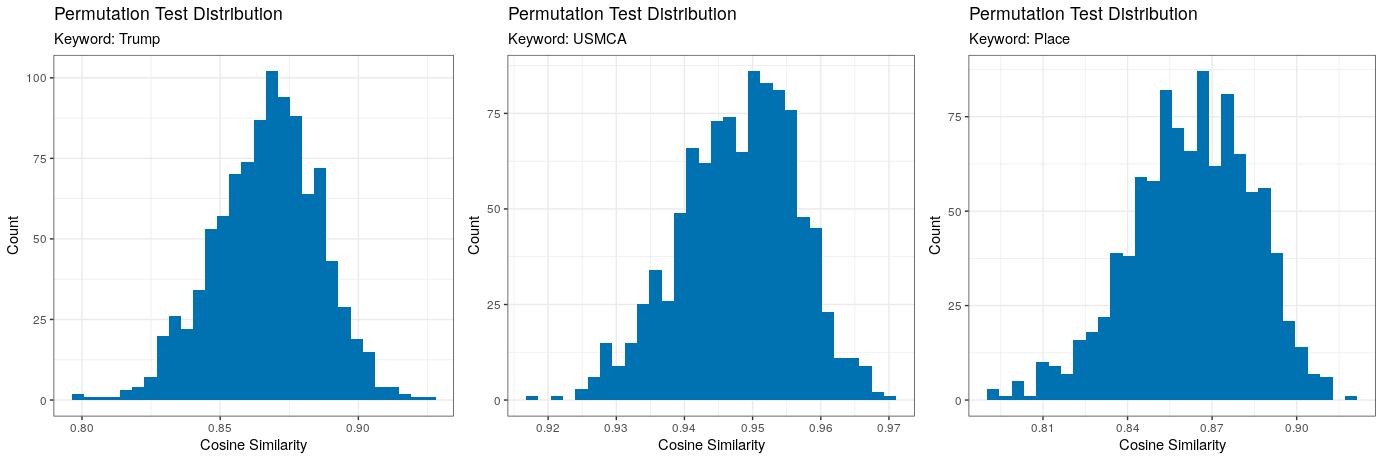
\includegraphics[width=1\textwidth]{permutation}
  \caption{Permutation test for key words}
  \label{fig:permutation}
\end{figure}

\begin{table}[h]
    \caption{Permutation test results}
    \begin{tabular}{lllllll}
      \toprule
        \multicolumn{4}{r}{Permutation}                   \\
        \cmidrule(r){3-6}
      Label    & Observed value & Mean & Min  & Max  & $\sigma$\\
      \midrule
      Trump    & 0.37           & 0.87 & 0.80 & 0.92 & 0.02 \\
      USMCA    & 0.67           & 0.95 & 0.92 & 0.97 & 0.01 \\
      Place    & 0.46           & 0.86 & 0.79 & 0.92 & 0.02 \\
      \bottomrule
    \end{tabular}
    \label{table:perm}
\end{table}

Figure \ref{fig:permutation} shows a histogram for each of the words tested and table \ref{table:perm} provides descriptive statistics. These results are in line with my hypothesis and provide strong evidence that word embeddings are capturing semantic differences between parties. Across all three words, none of the permuted distributions contained the observed value. Additionally, as expected the difference from the mean of the permuted labels and the observed value was greatest between the disagree word ``trump'' and smallest between the agree word ``usmca.''


\subsection{Hypothesis 3: If separate word vectors are calculated for ideologically distinct groups, the word vectors that represent points of disagreement will have a lower cosine similarity than those that represent points of agreement.}

My final hypothesis seeks to test the generalizability of the results from the second hypothesis. To do so, I calculated the cosine similarity for each word and its ideological counterpart in my list. I then calculate the mean cosine similarity for each of the three word groups. Figures \ref{fig:density} and \ref{fig:box} show the distribution of cosine similarity by category and table \ref{table:dist} provides descriptive statistics. 

\begin{figure} [h]
  \centering
  \subfigure[Cosine similarity density plot]{
  \label{fig:density}
  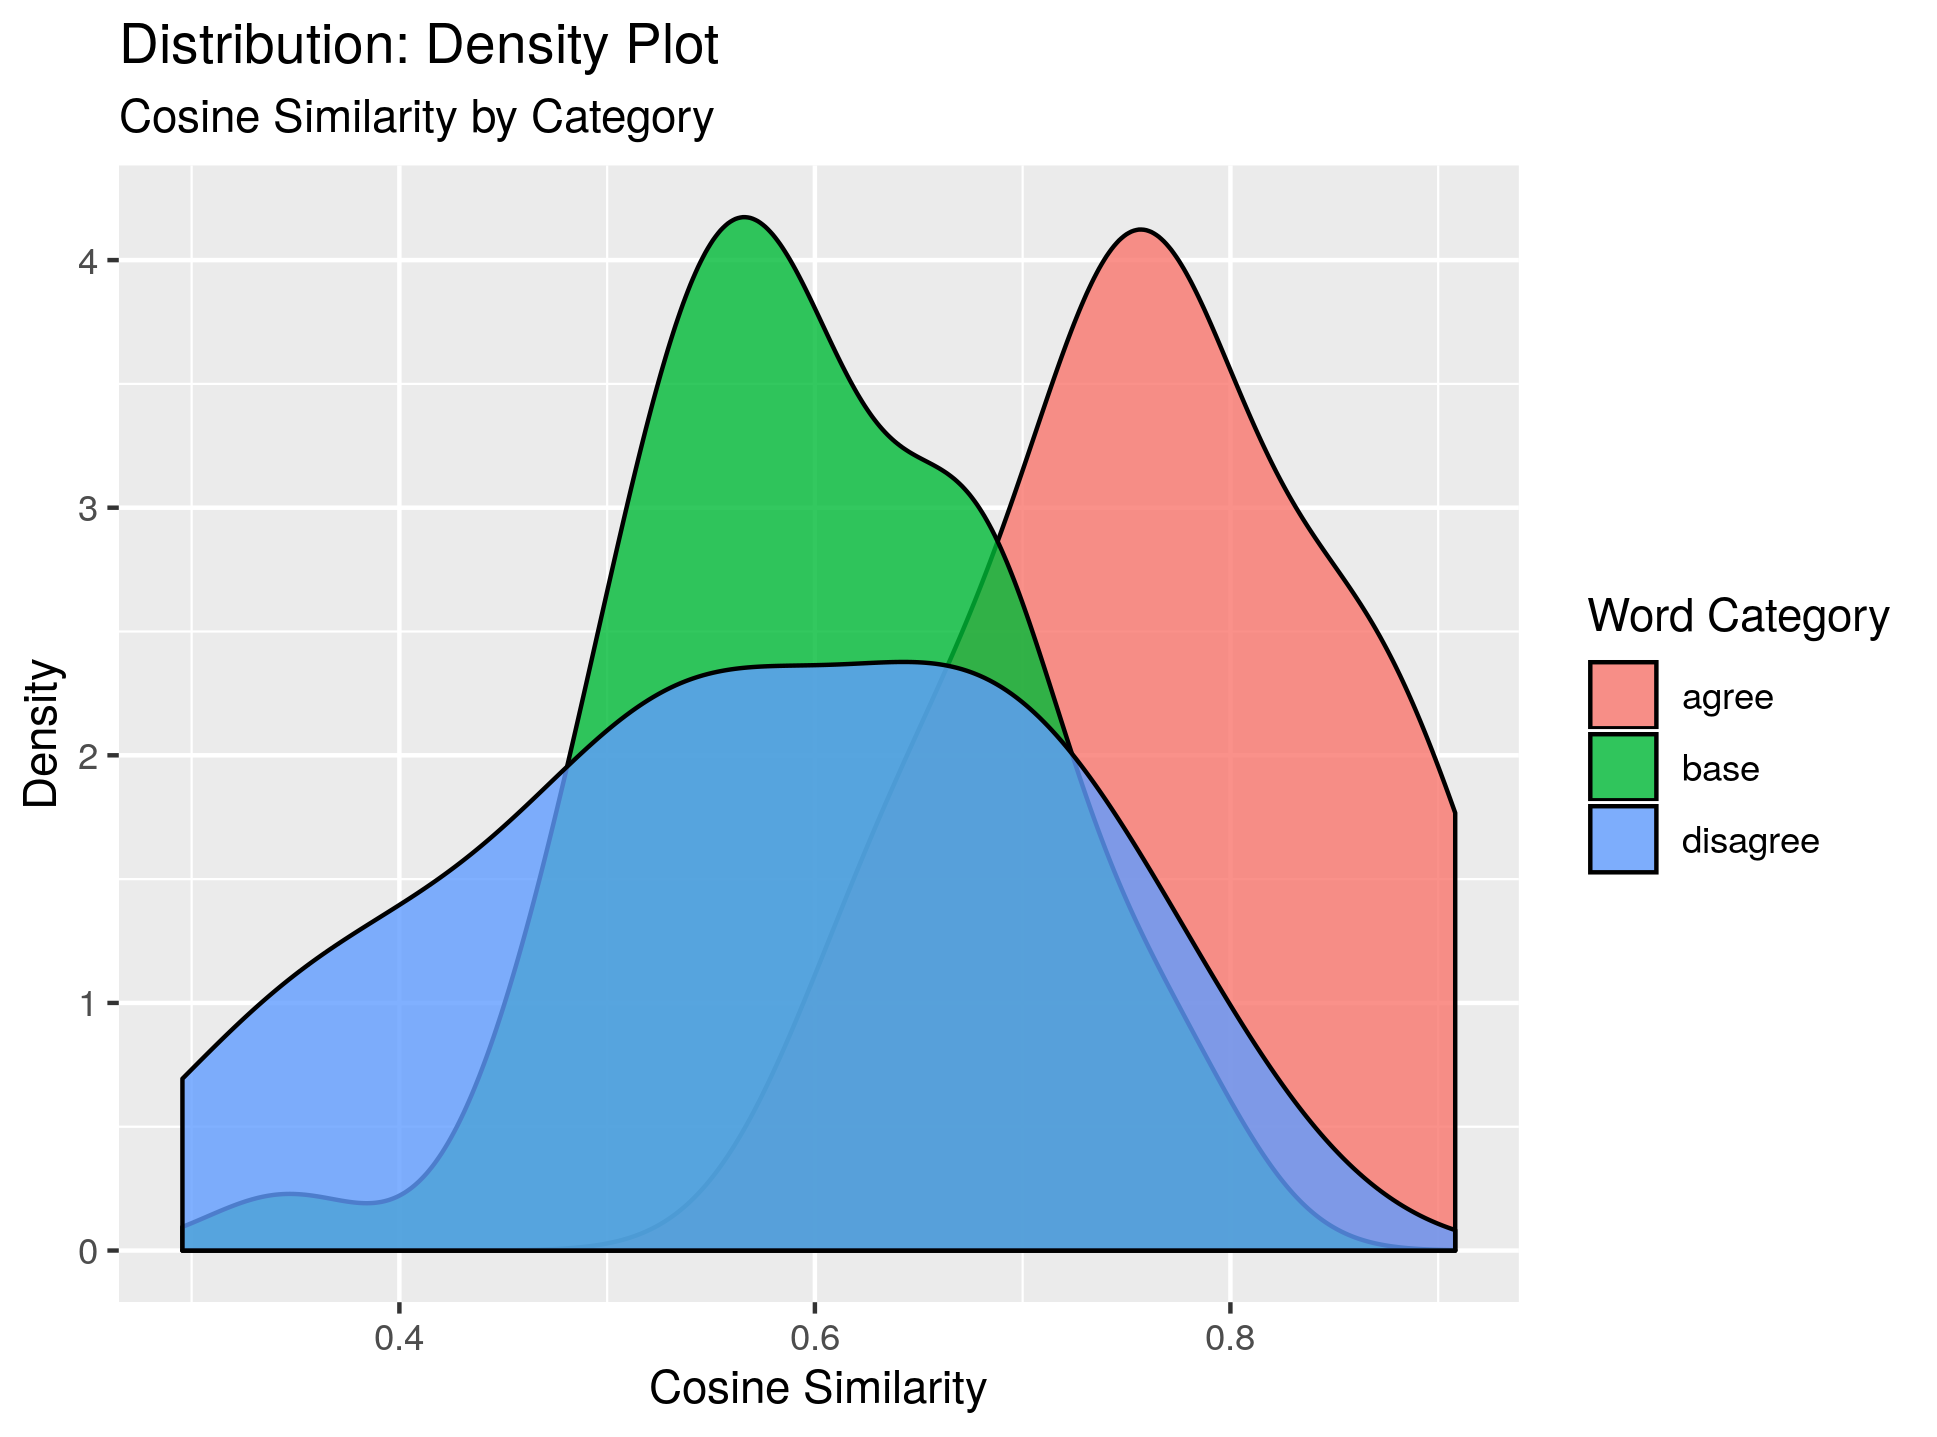
\includegraphics[width=.45\textwidth]{density}}
  \qquad
  \subfigure[Cosine similarity box plot]{
  \label{fig:box}
  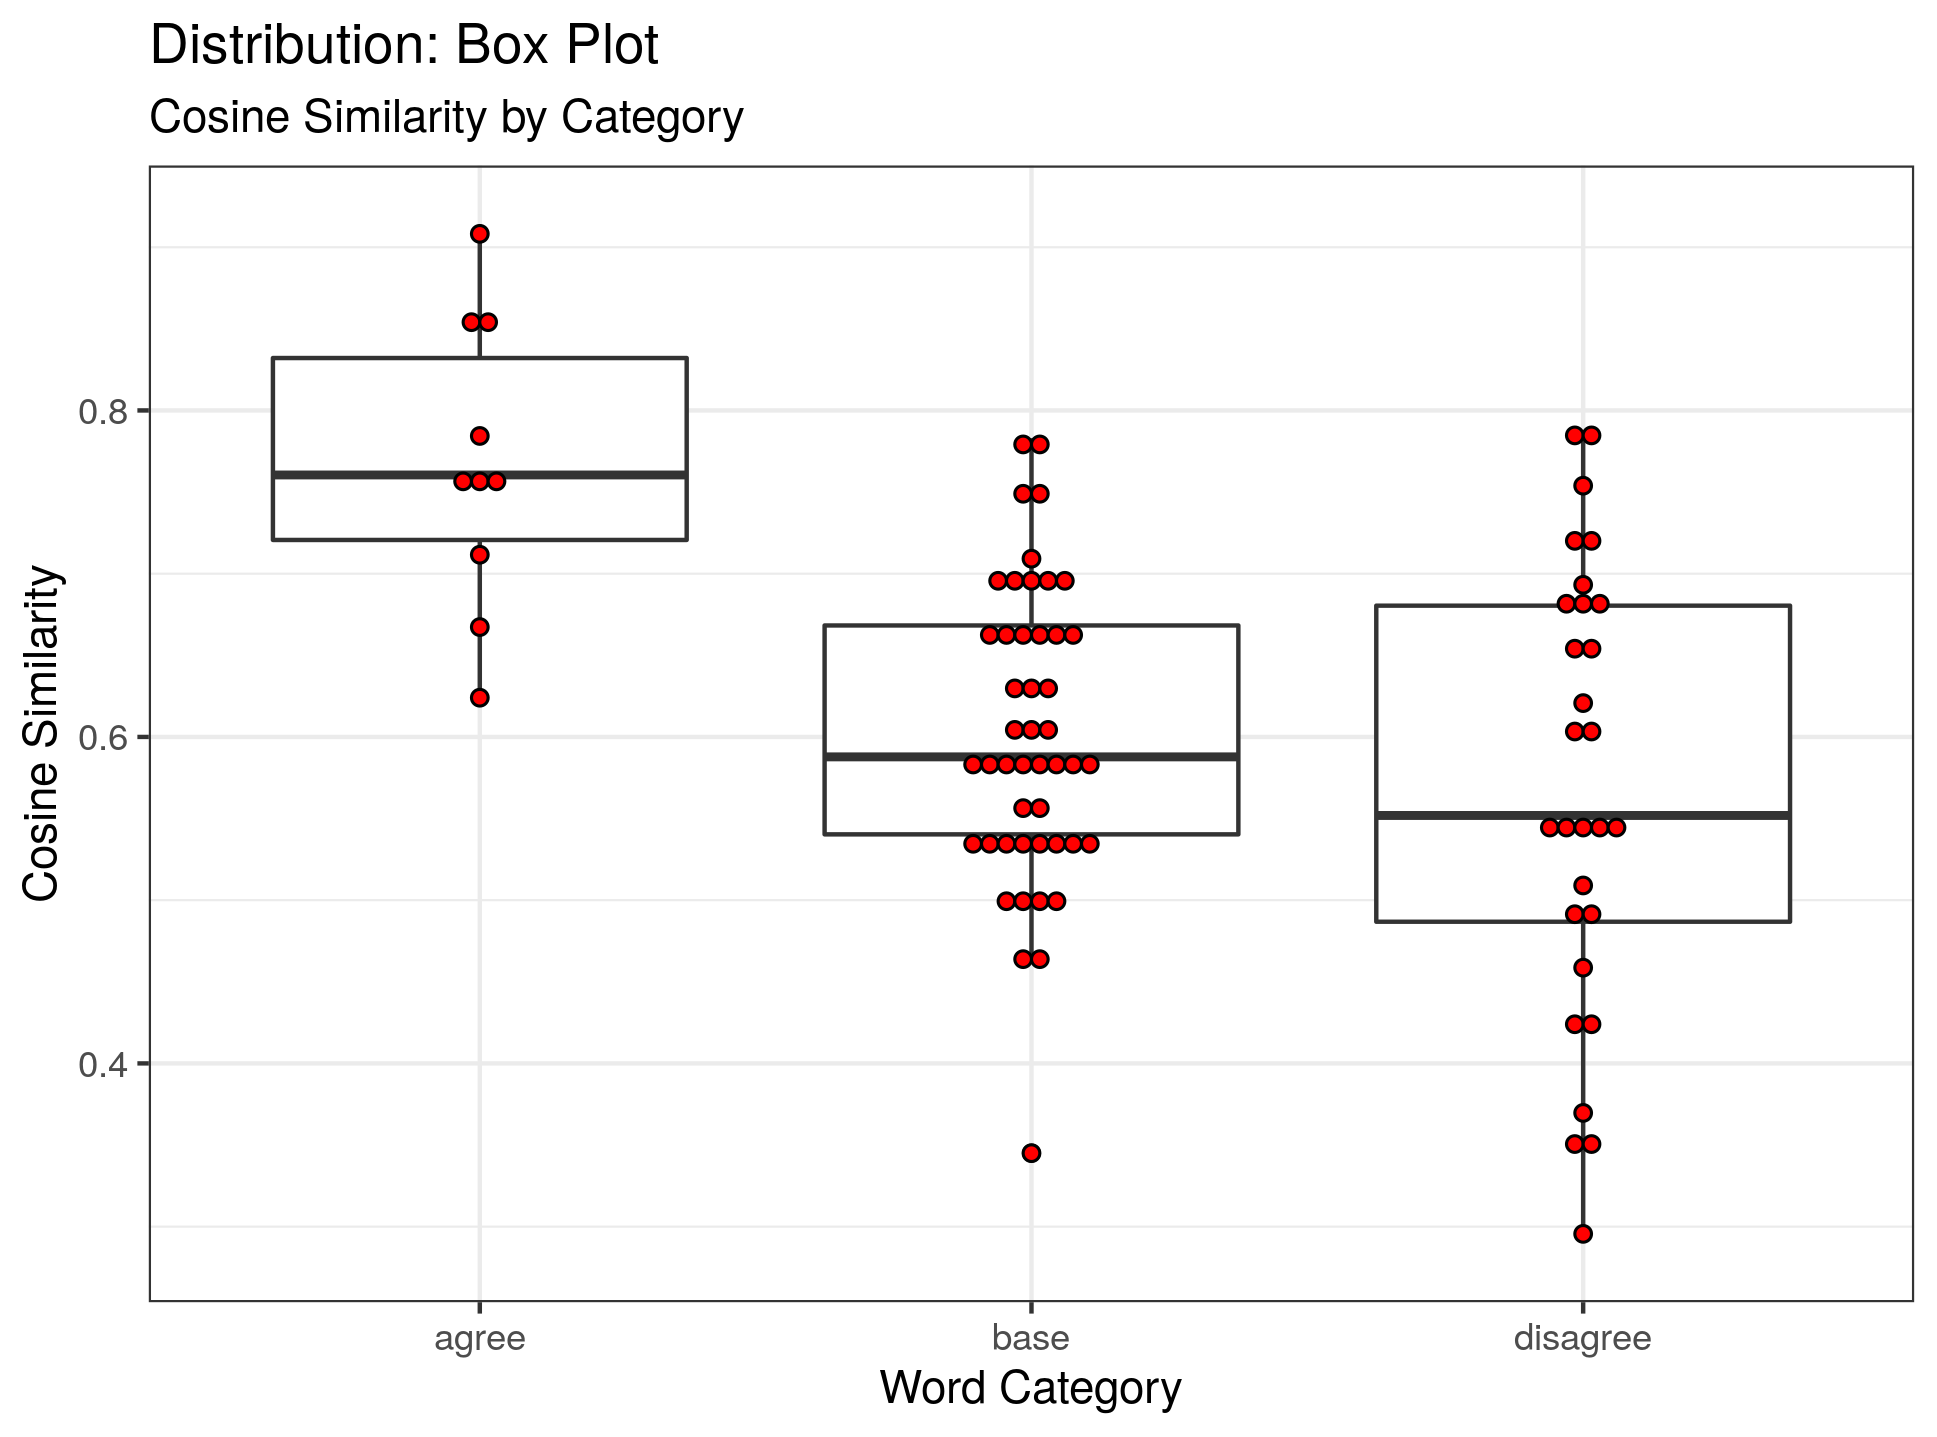
\includegraphics[width=.45\textwidth]{boxplot}}
  \caption{Distribution of cosine similarity by word category}
\end{figure}

\begin{table}[h]
    \caption{Distribution of cosine similarity by word category}
    \begin{tabular}{llllll}
      \toprule
      Label    & Mean & Min  & Max  & $\sigma$ & \textit{n}\\
      \midrule
      Disagree & 0.57 & 0.30 & 0.79 & 0.14   & 29\\
      Agree    & 0.77 & 0.62 & 0.91 & 0.09   & 10\\
      Base     & 0.60 & 0.35 & 0.78 & 0.09   & 47\\
      \bottomrule
    \end{tabular}
    \label{table:dist}
\end{table}

I use a difference of means test to evaluate differences between the groups. I expect that words in the disagree category will have the lowest cosine similarity, the agree category will have the highest, and non-ideological will be in the middle. Because the number of words is relatively small, I use a permutation test and a bootstrap confidence interval to supplement the t-test. Results are shown in table \ref{table:cs}. I consider these results to be generally inconclusive. The tests do reveal a consistent difference between the agree and disagree words, they do not clearly distinguish between the disagree words and the noise of the base words. This lack of distance between disagree and base words is an unexpected result. Base words are those that can be found in any context and generally carry no ideological significance. While some deviation between tese words and their counterparts is to be expected because Democrats and Republicans do not engage in the same topics of discussion with the same frequency, I expect these words to be relatively synonymous, and thus closer to the agree category. 

\begin{table}[h]
    \caption{Difference of means relative to disagree words}
    \begin{tabular}{lllll}
      \toprule
      Label    & Mean  & t-test (p) & Permutation (p) & Bootstrap (CI)\\
      \midrule
      Disagree & 0.57  & -          & -               & -\\
      Agree    & 0.77  & 2.11e-05   & 0.002           & (-0.27, -0.13)\\
      Base     & 0.60  & 0.29       & 0.23            & (-0.09, 0.02)\\
      \bottomrule
    \end{tabular}
    \label{table:cs}
\end{table}

There are perhaps two primary factors driving these inconclusive results. First are potential shortcomings in my list of terms. This is suggested by the relatively large standard deviation in cosine similarity among these words and a retroactive look at the text behind some of the outliers. For example, I selected the word ``police'' under the expectation that it would capture different attitudes on police brutality and the Black Lives Matter movement. Generally speaking however, elected officials seemed reluctant to criticize domestic law enforcement on social media. Additionally, Ongoing police brutality surrounding the Hong Kong protests has been denounced by both parties on social media. ``Police'' therefore did not capture the intended subject and instead captured one on which there is relative agreement. Similarly, the word ``healthcare'' was included in the disagree list but was probably more noise than signal. While there is certainly disagreement between the parties on healthcare, clear party platforms have not emerged and there is significant disagreement within the parties as well. Thus, I would probably need to draw different ideological boundaries to measure this particular concept. 

\begin{figure}[h]
  \centering
  \subfigure[Relative cosine similarity density plot]{
  \label{fig:rcsdensity}
  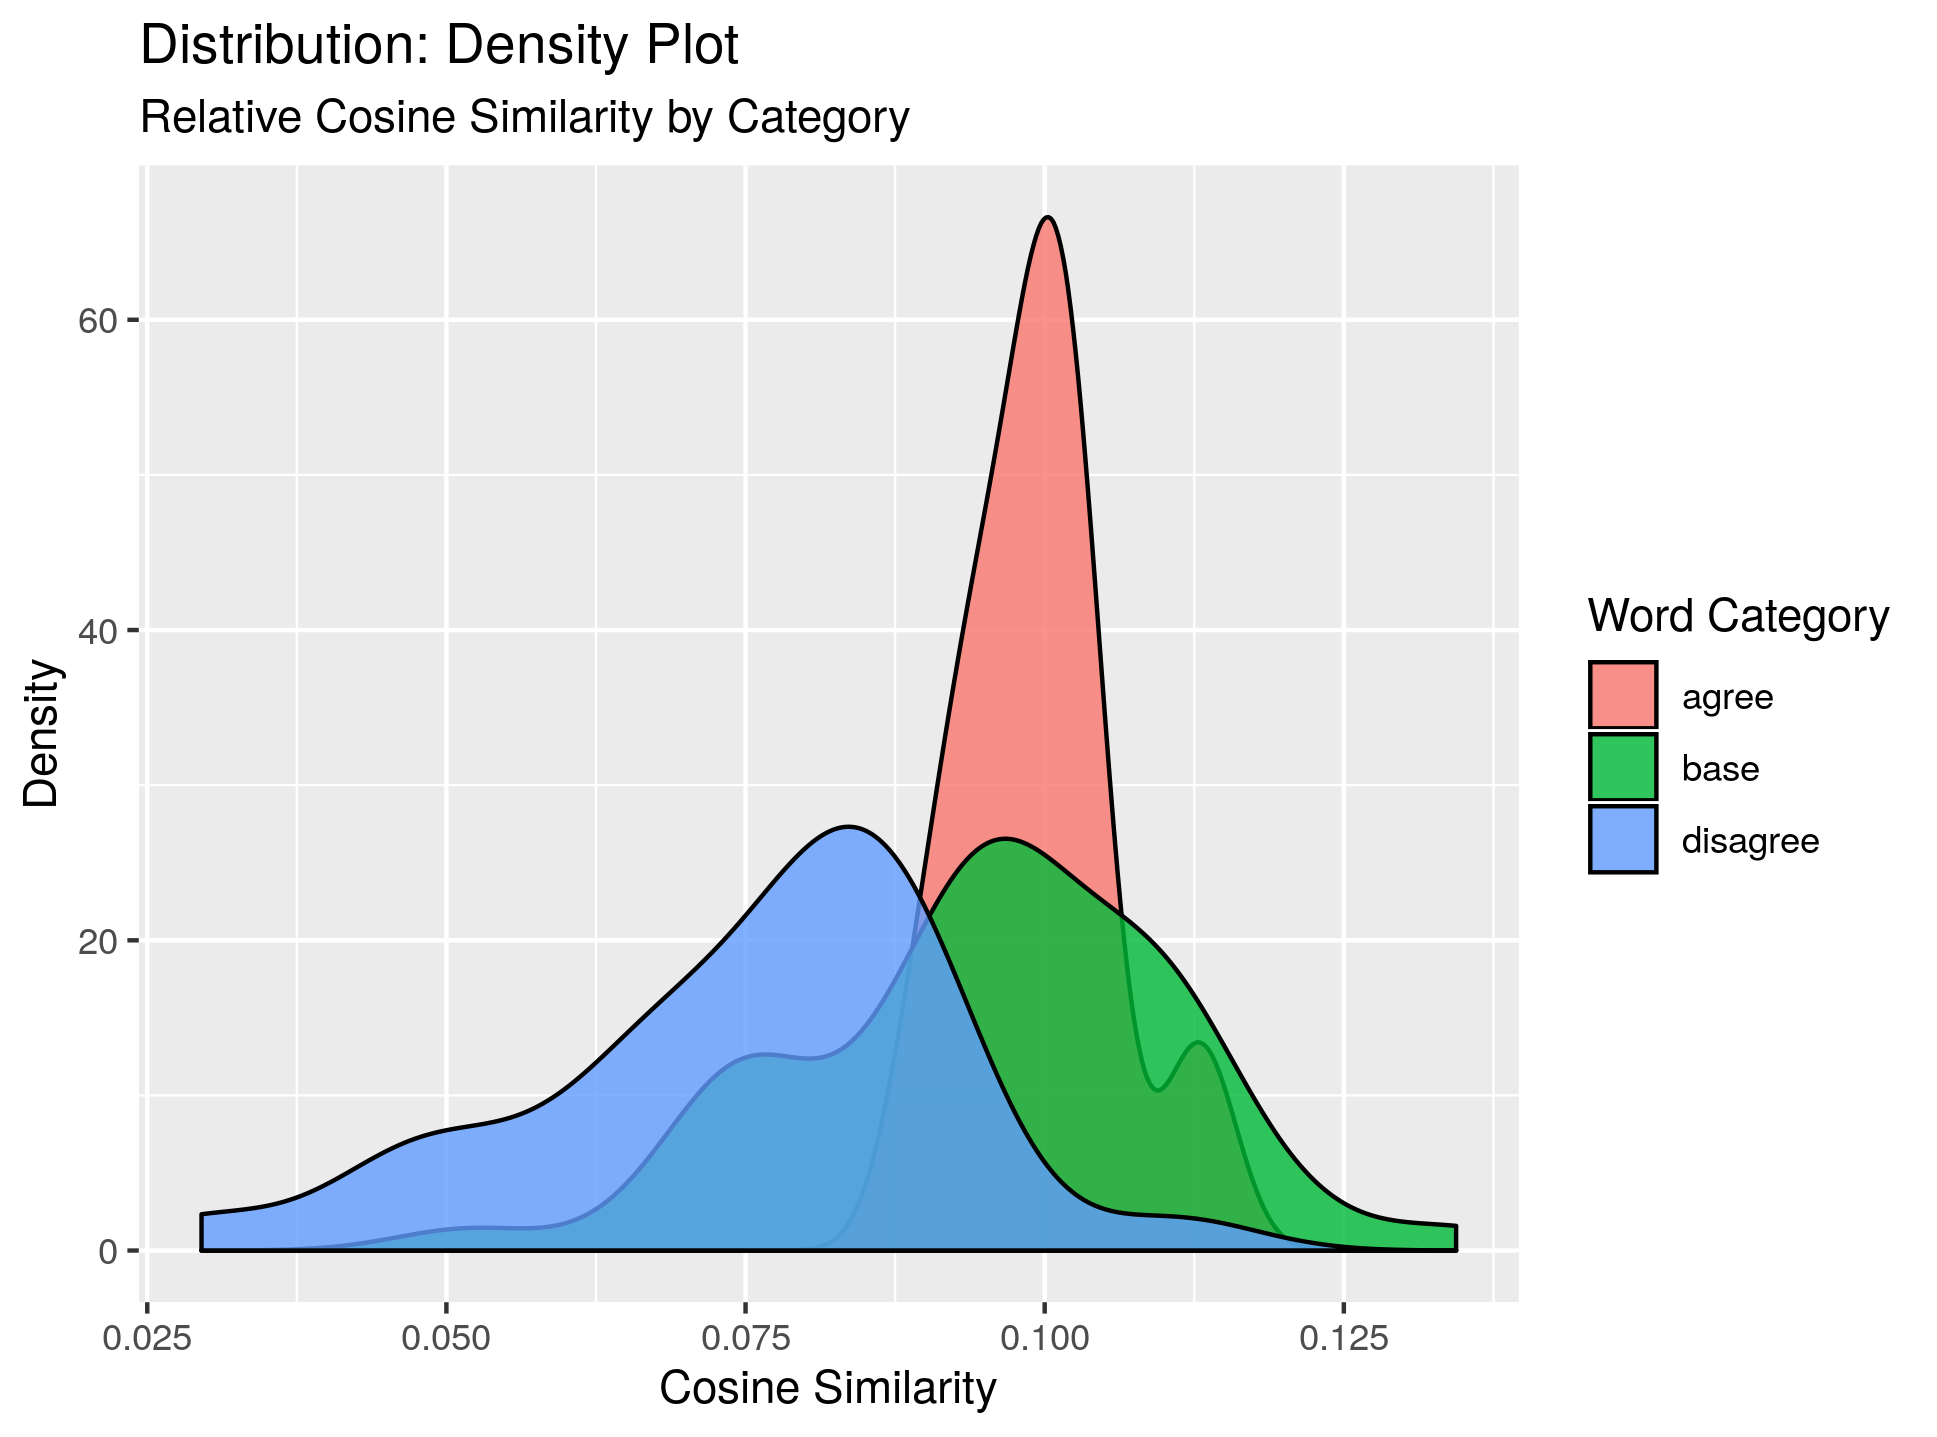
\includegraphics[width=.45\textwidth]{rcs_density}}
  \qquad
  \subfigure[Relative cosine similarity box plot]{
  \label{fig:rcsbox}
  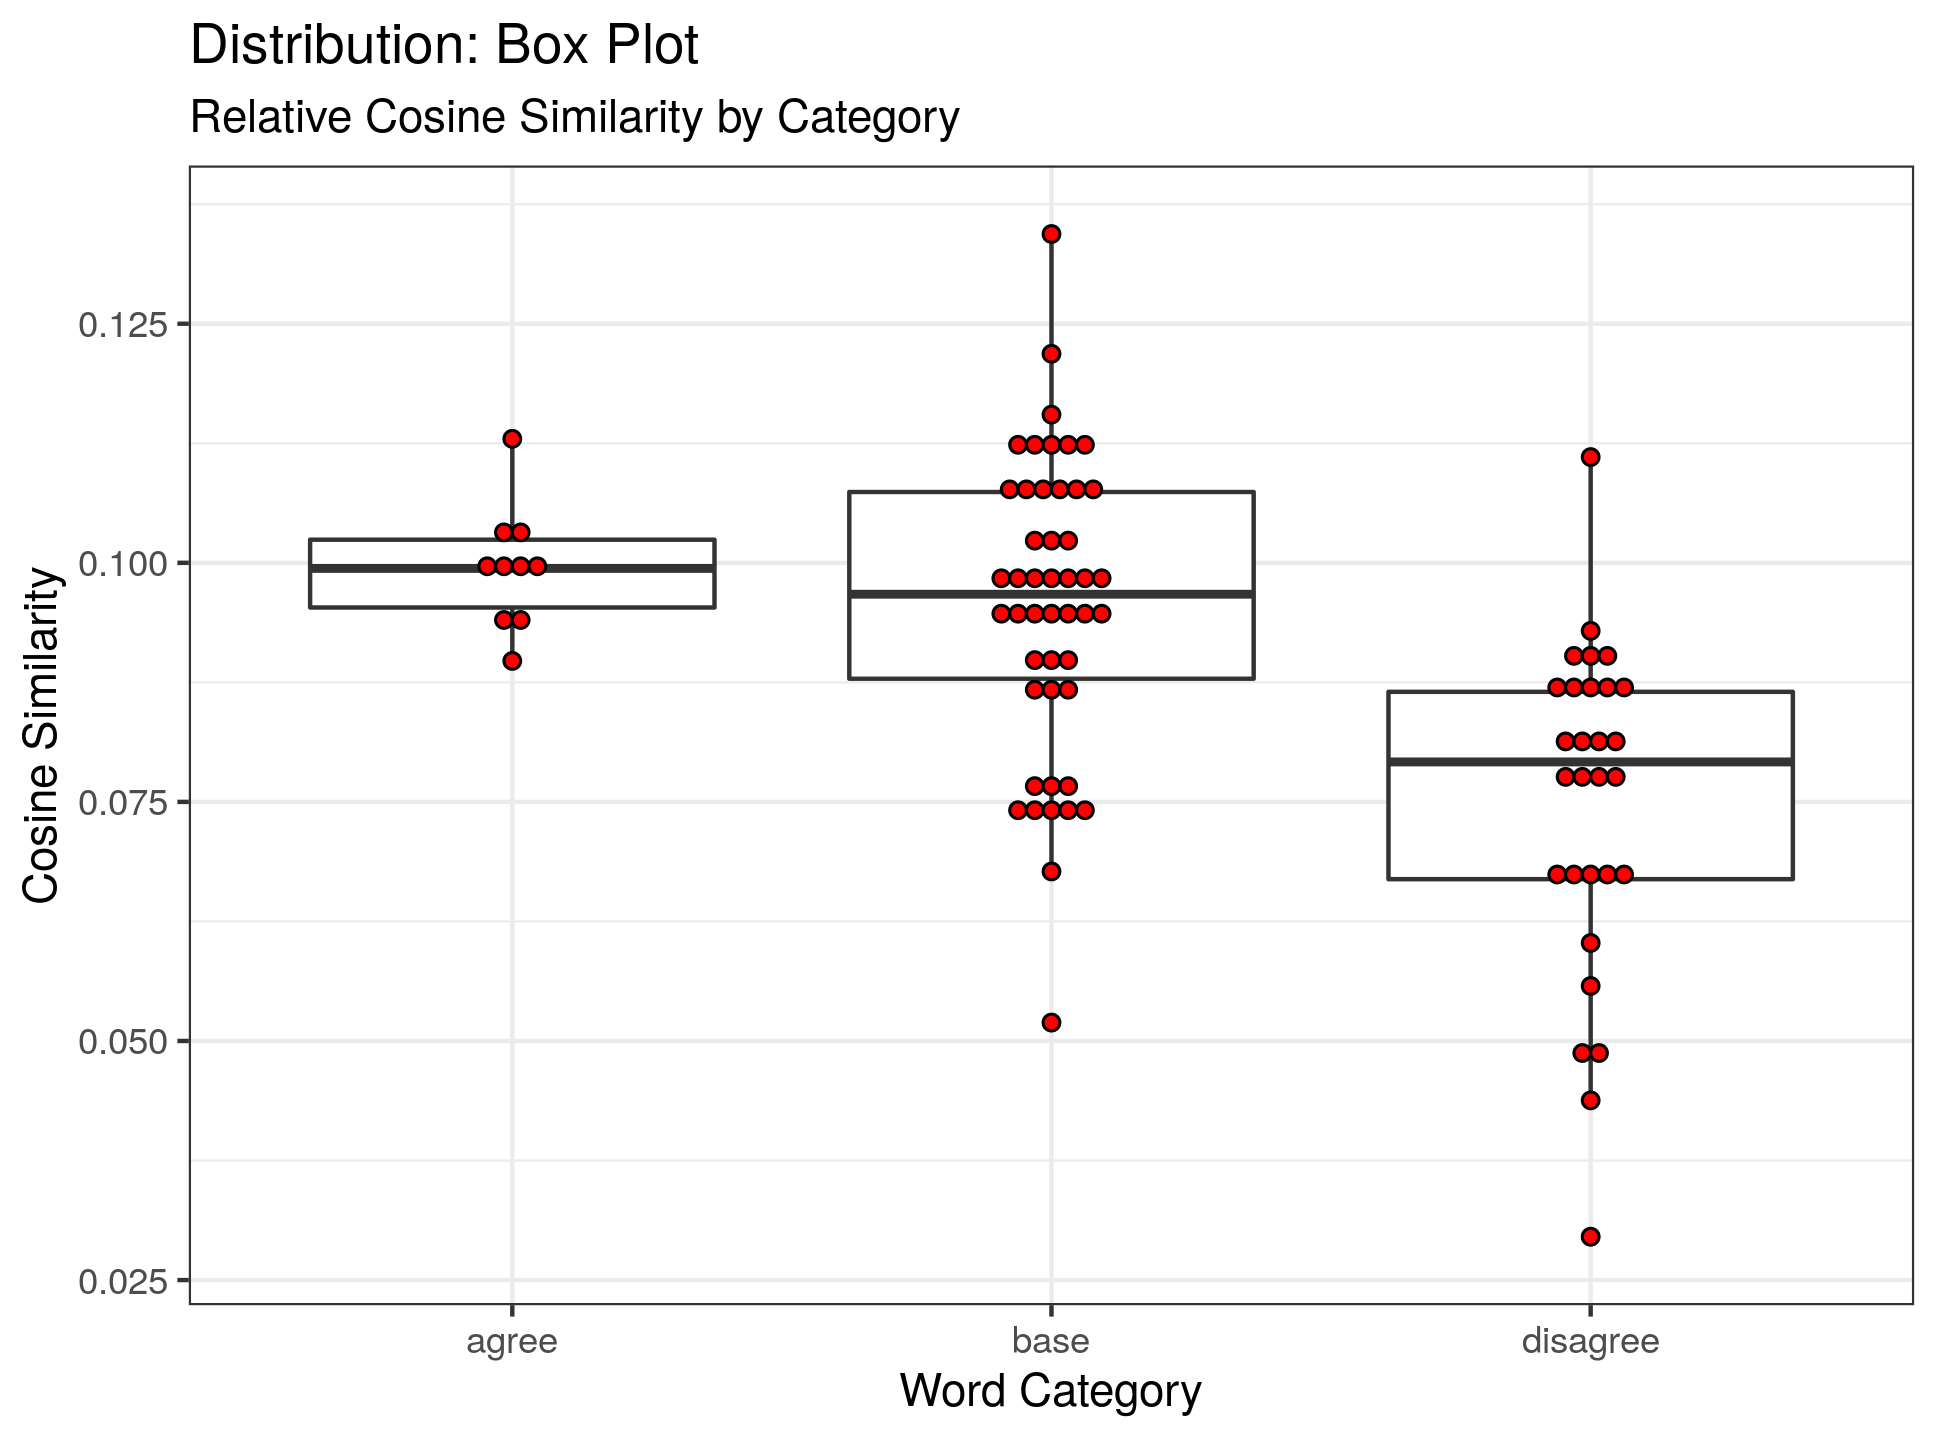
\includegraphics[width=.45\textwidth]{rcs_boxplot}}
  \caption{Distribution of relative cosine similarity by word category}
\end{figure}

\begin{table}[h]
    \caption{Distribution of cosine similarity by word category}
    \begin{tabular}{llllll}
      \toprule
      Label    & Mean  & Min   & Max  & $\sigma$ & \textit{n}\\
      \midrule
      Disagree & 0.075 & 0.030  & 0.111 & 0.017   & 29\\
      Agree    & 0.100 & 0.090  & 0.113 & 0.006   & 10\\
      Base     & 0.095 & 0.052 & 0.134 & 0.016   & 47\\
      \bottomrule
    \end{tabular}
    \label{table:rcsdist}
\end{table}

The second shortcoming is simply that cosine similarity is a bit of a blunt instrument. In their research on synonym extraction, Leeuwenberg et al. showed that cosine similarity alone is a bad indicator to determine if two words are synonymous. Instead, they propose a technique they call relative cosine similarity which examines the similarity between two words relative to other words in the corpus \cite{leeuwenberg2016minimally}.  Accordingly, I repeat the above analysis using relative cosine similarity. Figures \ref{fig:rcsdensity} and \ref{fig:rcsbox} show the distribution of the data and table \ref{table:rcsdist} provides descriptive statistics. As a rule of thumb, if relative cosine similarity is greater than 0.10, the two words are more similar than an arbitrary word pair \cite{rehurek_lrec}.



Relative cosine similarity produces results more in line with expectations than simple cosine similarity. Most notably, the significance in the difference between agree and disagree words increased and the base word category is now closer in proximity to the agree word category. 

\begin{table}[h]
    \caption{Difference of means relative to disagree words}
    \begin{tabular}{lllll}
      \toprule
      Label    & Mean  & t-test (p) & Permutation (p) & Bootstrap (CI)\\
      \midrule
      Disagree & 0.075  & -          & -               & -\\
      Agree    & 0.100  & 1.54e-07   & 0.002           & (-0.032, -0.017)\\
      Base     & 0.095  & 3.25e-06   & 0.002            & (-0.028, -0.013)\\
      \bottomrule
    \end{tabular}
    \label{table:rcs}
\end{table}

\end{document}